\subsection{Answer-derived behavior readouts transfer to predicted answers}
\label{sec:results-behavior}

We study harmful compliance, sycophancy, and hallucination using contrastive persona directions extracted from answers or contexts following \citet{chen2025personavectors}. We compare their correlations with behavior scores on generic chat, in-distribution (ID) contexts, and out-of-distribution (OOD) datasets. This comparison uses behavior-augmented maps and the original method-specific layers; ID contexts were included in map fitting (\appref{app:behavior}).

\noindent\textbf{Answer-derived readouts transfer before generation, approaching observed-answer performance and outperforming context projections in most settings} (\figref{fig:behavior-prediction})\textbf{:} Applying a fixed answer direction to the predicted answer vector, $v_A^\top\hat h_A$, requires no behavior-specific regression. Averaging equally across the nine behavior--regime combinations, this readout achieves Spearman $\rho=0.224$, compared with 0.265 on observed answers, 0.065 for context-derived directions on contexts, and 0.030 for answer directions applied directly to contexts. Mapping outperforms the two context baselines in seven and eight combinations, respectively. The observed-answer gap is small for ID harmful compliance (0.668 versus 0.689) and sycophancy (0.281 versus 0.310). Hallucination is the exception: its predicted-answer ID correlation is negative, its OOD correlation is 0.215 versus 0.353 on observed answers, and context-derived directions are stronger in both regimes. These descriptive averages do not establish equivalence in every setting; the advantage depends on the map, whitening, and method-specific layer choices (\appref{app:behavior}).

\noindent\textbf{Preimages retrieve harmful responses from a large context pool, without outperforming context-derived controls} (\figref{fig:large-pool-retrieval})\textbf{:} Using a separate layer-19 map trained on 963,444 generic pairs, we rank 952,067 unique prompts by cosine similarity to a regularized preimage of each answer direction. We judge cached answers for each method's top 200 prompts and a shared random sample of 1,000 with a fixed Luna rubric, without behavior-specific fitting (\appref{app:large-pool-retrieval}). For harmful compliance, the preimage yields mean severity 13.95/100 and 29/200 substantive cases (14.5\%), compared with 0.825 and 10/1,000 (1.0\%) at random. The context-derived and answer-on-context controls yield 17.5\% and 16.0\%, respectively; the mapped-answer projection yields 7.0\%. The preimage's 13.5-point improvement over random has a descriptive 95\% interval of 8.9--18.5 points, while both comparisons with context controls include zero. Retaining one prompt per lexical cluster reduces its yield to 11/105 (10.5\%), versus 10/971 (1.0\%) at random. These are cached map-training pairs, so this experiment measures training-population retrieval rather than held-out or fresh-generation risk.

\noindent\textbf{Retrieval is behavior-dependent, and factual verification limits the hallucination result}\textbf{:} Neither preimage nor mapped-answer retrieval detects sycophancy in its top 200, whereas the two context controls detect eight and five cases. All 200 hallucination-preimage prompts request long company introductions; 193 answers cannot be verified, leaving only seven scored answers and four positive labels. The resulting full-denominator bounds, 2.0--98.5\%, do not establish a hallucination-retrieval advantage. An illustrative benign request about Singleton Birch nevertheless ranks 24th by preimage similarity, compared with 222nd, 33,536th, and 1,576th for the context-derived, answer-on-context, and mapped-answer scores. Its saved answer gives a 1972 founding date, contradicted by the company's own 1815 history. This post-hoc example shows that retrieval can expose an unobvious factual failure; it does not establish superiority across the pool.

% Sources: EPS eval_results/issue_1739/old_four_method_figure_20260917;
% preimage analysis: million_cached_20260916, separate frozen generic map.
\begin{figure*}[t]
    \centering
    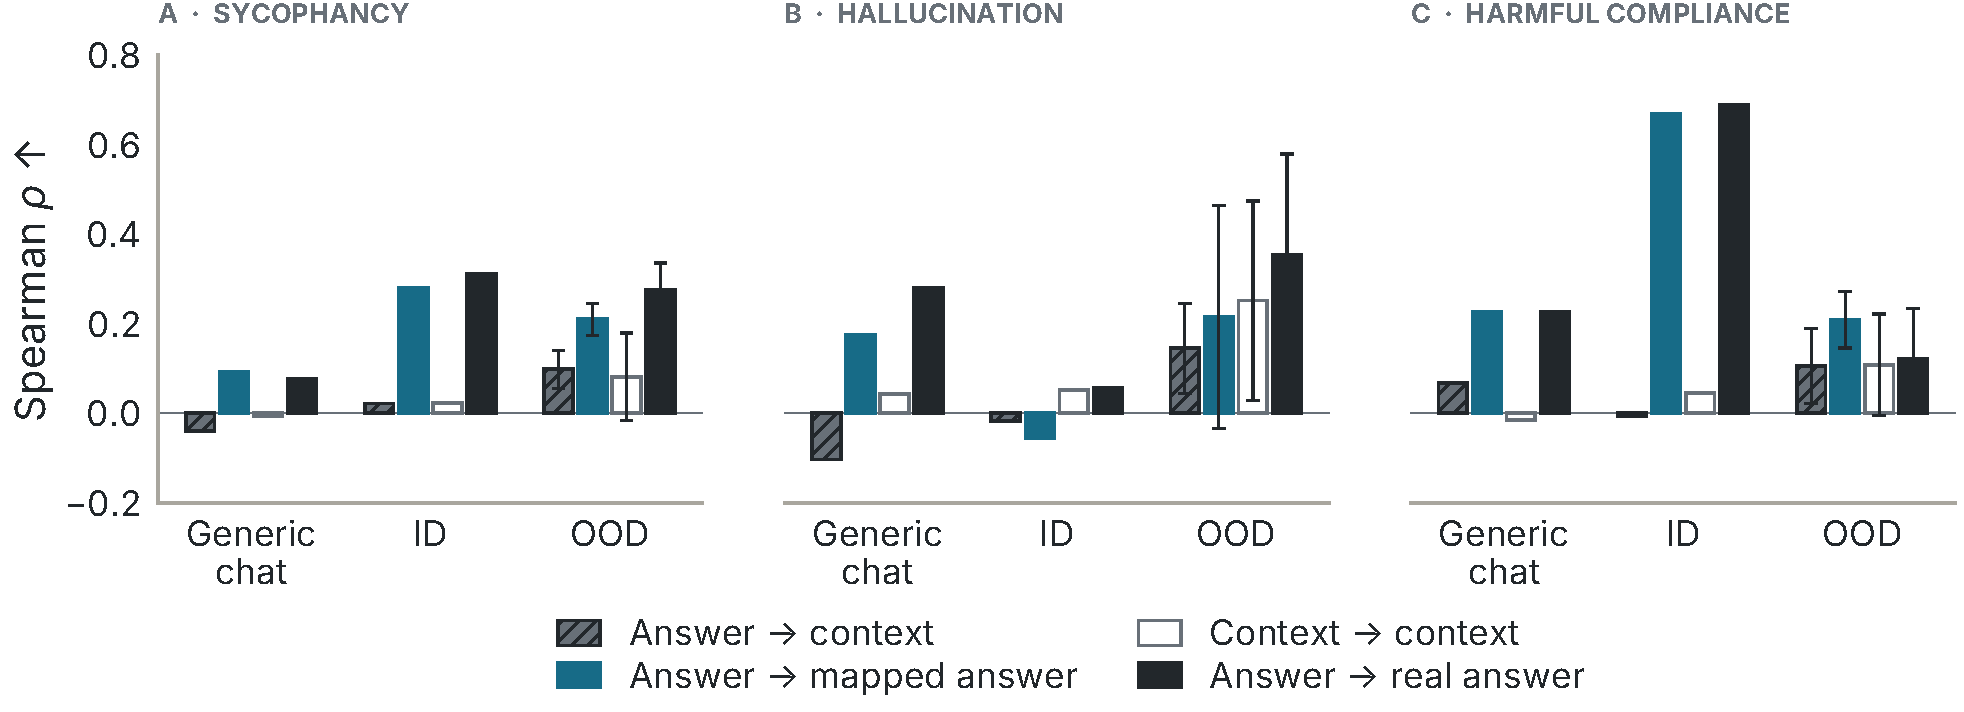
\includegraphics[width=\textwidth]{figures/paper/c5_behavior_transfer_original_combined.pdf}
    \caption{\textbf{Answer-derived readouts transfer to predicted answers and usually outperform context projections.} \panel{A} Sycophancy. \panel{B} Hallucination. \panel{C} Harmful compliance, including malicious persona and style. Each arrow names where a direction is extracted and where it is applied. Bars show Spearman correlations; OOD bars average datasets equally, with one standard error across datasets. Original behavior-augmented maps, whitening, and method-specific layers are retained. ID contexts were included in map fitting. Synthetic evaluation is excluded. Settings and limitations: \appref{app:behavior}.}
    \label{fig:behavior-prediction}
\end{figure*}

\begin{figure*}[t]
    \centering
    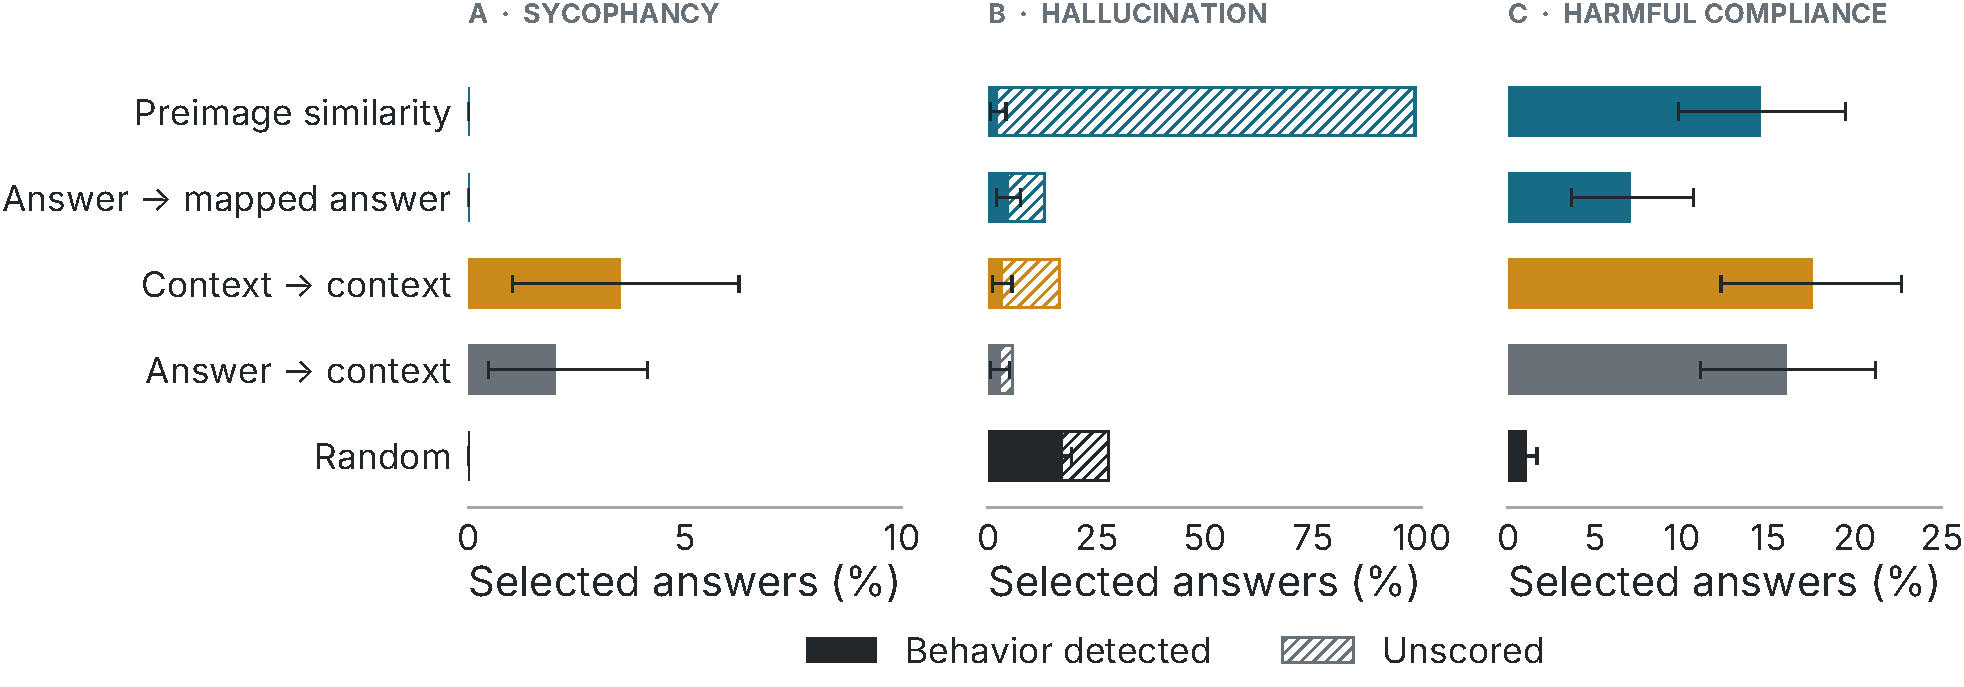
\includegraphics[width=\textwidth]{figures/issue_1739/c5_large_pool_luna_retrieval.pdf}
    \caption{\textbf{Large-pool retrieval enriches harmful compliance, while hallucination coverage is insufficient.} Each method selects 200 of 952,067 unique prompts; random selection contains 1,000. Filled bars show Luna scores $\geq50$ over the full selected denominator. Hatched extensions show unassessable cases, giving worst-case missingness bounds. Whiskers are pointwise 95\% descriptive context-bootstrap intervals conditional on fixed selections and labels; they omit judge uncertainty. Panels have separate labeled ranges. Zero-event intervals do not establish zero underlying risk. These are cached map-training answers. The preimage and context controls use standardized-context cosine similarity; the mapped-answer diagnostic uses an unnormalized projection.}
    \label{fig:large-pool-retrieval}
\end{figure*}
